% In questo file vengono definiti comandi (macro) utili in tutti i documenti

\newcommand{\gruppo}{\textit{Sirius}} % nome gruppo
\newcommand{\progetto}{\textit{Sequenziatore}} % nome progetto
\newcommand{\capitolato}{\href{http://www.math.unipd.it/~tullio/IS-1/2013/Progetto/C4p.pdf}{http://www.math.unipd.it/~tullio/IS-1/2013/Progetto/C4p.pdf}} 

% GLOSSARIO
\newcommand{\lastversionG}{4.0.0}
\newcommand{\Glossario}{\textit{Glossario\_{}v\lastversionG{}.pdf}}
\newcommand{\doctitleG}{Glossario}
\newcommand{\infoG}{\doctitleG\ v\lastversionG}

% NORME DI PROGETTO
\newcommand{\lastversionNDP}{4.0.0}
\newcommand{\NormeDiProgetto}{\textit{NormeDiProgetto\_{}v\lastversionNDP{}.pdf}}
\newcommand{\doctitleNDP}{Norme di progetto}
\newcommand{\infoNDP}{\doctitleNDP\ v\lastversionNDP}

% ANALISI DEI REQUISITI
\newcommand{\lastversionAR}{3.0.0}
\newcommand{\AnalisiDeiRequisiti}{\textit{AnalisiDeiRequisiti\_{}v\lastversionAR{}.pdf}}
\newcommand{\doctitleAR}{Analisi dei requisiti}
\newcommand{\infoAR}{\doctitleAR\ v\lastversionAR}

% Studio di fattibilita
\newcommand{\lastversionSDF}{2.0.0}
\newcommand{\StudioDiFattibilita}{\textit{StudioDiFattibilita\_{}v\lastversionSDF{}.pdf}}
\newcommand{\doctitleSDF}{Studio Di Fattibilità}
\newcommand{\infoSDF}{\doctitleSDF\ v\lastversionSDF}

% Piano di qualifica
\newcommand{\lastversionPDQ}{4.0.0}
\newcommand{\PianoDiQualifica}{\textit{PianoDiQualifica\_{}v\lastversionPDQ{}.pdf}}
\newcommand{\doctitlePDQ}{Piano Di Qualifica}
\newcommand{\infoPDQ}{\doctitlePDQ\ v\lastversionPDQ}

% VERBALE 2014-02-03
\newcommand{\lastversionVb}{2.0.0}
\newcommand{\VerbaleB}{\textit{Verbale2014-02-03\_{}v\lastversionVb{}.pdf}}
\newcommand{\doctitleVb}{Verbale 2014-02-03}
\newcommand{\infoVb}{\doctitleVb\ v\lastversionVb}

% VERBALE 2014-07-20
\newcommand{\lastversionVN}{1.0.0}
\newcommand{\VerbaleN}{\textit{Verbale2014-07-20\_{}v\lastversionVN{}.pdf}}
\newcommand{\doctitleVN}{Verbale 2014-07-20}
\newcommand{\infoVN}{\doctitleVN\ v\lastversionVN}

%Piano di progetto
\newcommand{\lastversionPDP}{4.0.0}
\newcommand{\PianoDiProgetto}{\textit{PianoDiProgetto\_{}v\lastversionPDP{}.pdf}}
\newcommand{\doctitlePDP}{Piano Di Progetto}
\newcommand{\infoPDP}{\doctitlePDP\ v\lastversionPDP}
%Specifica Tecnica
\newcommand{\lastversionST}{3.0.0}
\newcommand{\SpecificaTecnica}{\textit{SpecificaTecnica\_{}v\lastversionST{}.pdf}}
\newcommand{\doctitleST}{Specifica Tecnica}
\newcommand{\infoST}{\doctitleST\ v\lastversionST}
%Definizione di prodotto
\newcommand{\lastversionDP}{2.0.0}
\newcommand{\DefinizioneDiProdotto}{\textit{DefinizioneDiProdotto\_{}v\lastversionDP{}.pdf}}
\newcommand{\doctitleDP}{Definizione Di Prodotto}
\newcommand{\infoDP}{\doctitleDP\ v\lastversionDP}

% MANUALE UTENTE
\newcommand{\lastversionMU}{2.0.0}
\newcommand{\ManualeUtente}{\textit{ManualeUtente\_{}v\lastversionMU{}.pdf}}
\newcommand{\doctitleMU}{Manuale utente}
\newcommand{\infoMU}{\doctitleMU\ v\lastversionMU}

% MANUALE PROCESS OWNER
\newcommand{\lastversionMPO}{2.0.0}
\newcommand{\ManualePO}{\textit{ManualeProcessOwner\_{}v\lastversionMPO{}.pdf}}
\newcommand{\doctitleMPO}{Manuale process owner}
\newcommand{\infoMPO}{\doctitleMPO\ v\lastversionMPO}
\newcommand{\lastversion}{\lastversionST}%versione del documento
\newcommand{\doctitle}{\doctitleST}%nome documento
\newcommand{\info}{\infoST}
\documentclass[11pt,a4paper]{article}
\usepackage[a4paper,portrait,top=3.5cm,bottom=3.5cm,left=3cm,right=3cm,bindingoffset=5mm]{geometry}


\usepackage[italian]{babel}
\usepackage{ucs} %unicode sistema gli accenti
\usepackage[utf8x]{inputenc} %unicode sistema gli accenti
\usepackage{fancyhdr}
\usepackage{subfigure} % per figure affiancate
\usepackage{hyperref}
\usepackage{float} % per far bene le figures
\usepackage{indentfirst}
\usepackage{longtable}
\usepackage{color}
\usepackage{colortbl}
\usepackage{rotating}
\usepackage[table]{xcolor}
\usepackage{wrapfig}
\usepackage{array}
\usepackage{eurosym}
\usepackage{graphicx}
\usepackage{breakurl}
\usepackage{lastpage} % total page count
\usepackage{chngpage}
\usepackage{amsfonts}
\usepackage{listings}
\usepackage{bookmark} % custom bookmarks

%\graphicspath{{./Pics}} % cartella di salvataggio immagini

% Per l'indice analitico
%\usepackage{makeidx}
%\makeindex

%pagestyle{fancy}
%\renewcommand{\chaptermark}[1]{\markboth{\thechapter.\ #1}{}}
%\renewcommand{\sectionmark}[1]{\markright{\thesection.\ \ #1}{}}
%\fancyhead{}
%comandi dell header
%\fancyhead[EL]{\slshape \leftmark}
%\fancyhead[OR]{\slshape \rightmark}
%\fancyfoot[EC,OC]{\slshape \thepage}

\pagestyle{fancy}
%\newcommand{\license}{\href{http://creativecommons.org/licenses/by/3.0/}{Some rights reserved}}
\newcommand{\groupname}{Sirius - Sequenziatore}

\newcommand{\subscript}[1]{\raisebox{-0.6ex}{\scriptsize #1}}
%\newcommand{\subscript}[1]{\ensuremath{_{\textrm{#1}}}}
%\renewcommand{\sectionmark}[1]{\markright{\thesection.\ #1}}
%\lhead{\nouppercase{\rightmark}}
%\rhead{\nouppercase{\leftmark}}
%\renewcommand{\chaptermark}[1]{\markboth{\thechapter.\ #1}{}}


\fancypagestyle{plain}{%
	\chead{}
	\lfoot{\info}
	\cfoot{}
	\rfoot{\thepage\ / \pageref{LastPage}}
	\renewcommand{\headrulewidth}{0.3pt}
	\renewcommand{\footrulewidth}{0.3pt}
}
	\lhead{\setlength{\unitlength}{1mm}
        \begin{picture}(0,0)
                \put(5,0){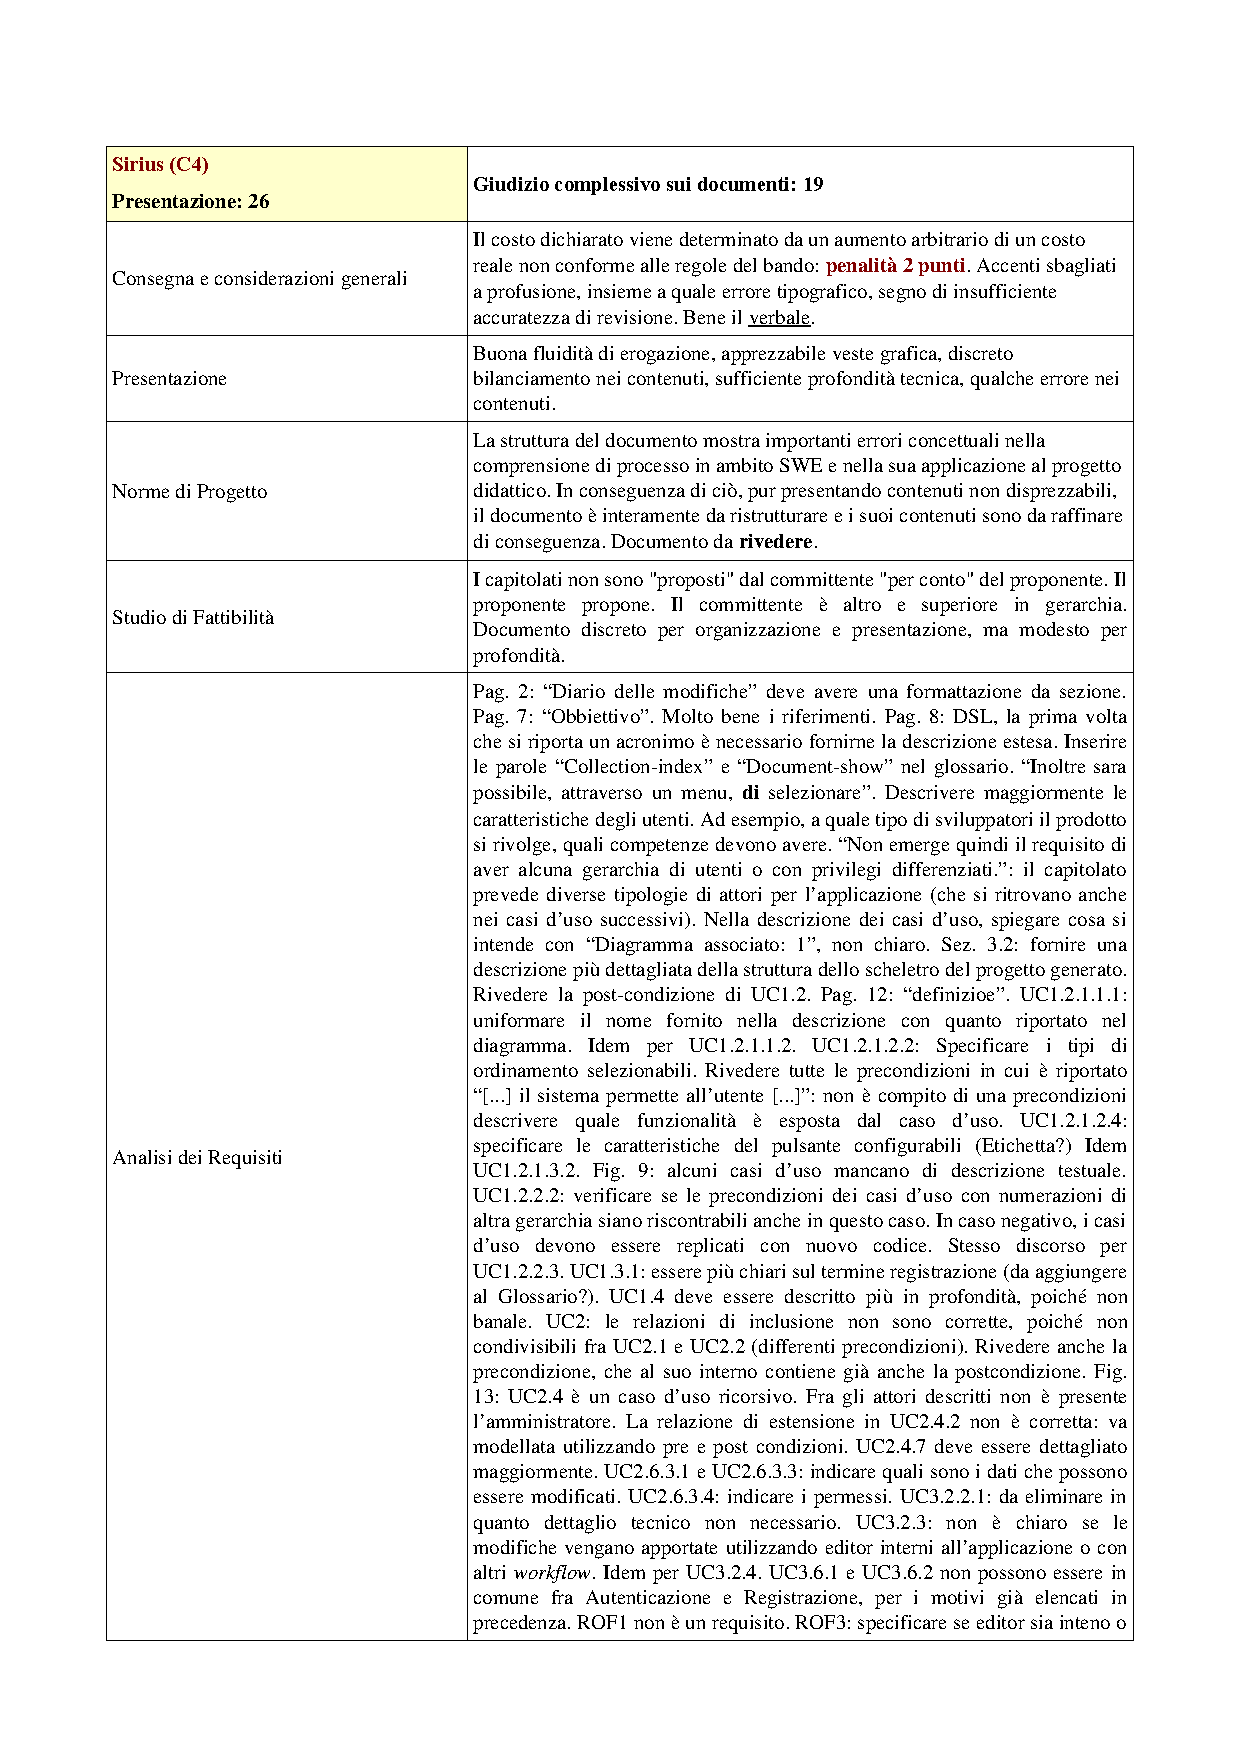
\includegraphics[scale=0.001]{img/Sirius.png}}
        \end{picture}}
	\rhead{\groupname}
	\chead{}
	\lfoot{\info}
	\cfoot{}
%	\rfoot{\thepage}
	\rfoot{\thepage\ / \pageref{LastPage}}
	\renewcommand{\headrulewidth}{0.3pt}
	\renewcommand{\footrulewidth}{0.3pt}
\linespread{1.2}	% valore interlinea


\fancypagestyle{romano}{
	\lhead{\setlength{\unitlength}{1mm}
        \begin{picture}(0,0)
                \put(5,0){
\includegraphics[scale=0.03]{../modello/img/sirius.png}}
        \end{picture}}
	\chead{}
	\rhead{\groupname}
	\lfoot{\info}
	\cfoot{}
	\rfoot{\thepage}
	\renewcommand{\headrulewidth}{0.3pt}
	\renewcommand{\footrulewidth}{0.3pt}
}



\hypersetup{
    colorlinks=true,linkcolor=[rgb]{0.11,0.55,0.83
    },          % colore link interni
    urlcolor=cyan           %colore link esterni
}
\definecolor{err}{rgb}{0.9,0.1,0.1}
\definecolor{rt}{rgb}{0.1,0.6,0.8}
\definecolor{grey}{rgb}{0.4,0.3,0.4}
\definecolor{mycolor}{rgb}{0.67,1,0.18}

\bibliographystyle{plain_ita}%bibliografia stile italiano

\pagenumbering{Roman}
\setlength\parindent{0pt} % sempre senza indentatura
% fine layout% layout
\begin{document}
% Prima pagina di opgni documento
\begin{titlepage}
 \begin{center}
     
\includegraphics[width=11cm]{../modello/img/sirius}\\
     \vspace{1em}
     {\LARGE \textsc{Sirius}}\\
     \vspace{2em} \hrule \vspace{2em}
     {\Large \textsc{Sequenziatore}}\\
     \vspace{8em}
     {\LARGE \LARGE \LARGE \textbf{\doctitle}}\\
     \vspace{2em}
     {\LARGE \LARGE \LARGE \textbf{Versione \lastversion }}\\
     \vspace{4em}
 \end{center}


\vskip 1.8cm
\begin{center}
\textit{Ingegneria Del Software AA 2013-2014}
\end{center}

\end{titlepage}


%pagina del titolo
\thispagestyle{romano}
\noindent\begin{Large}\textbf{Informazioni documento}\end{Large}\\
\begin{center}
\begin{tabular}{ll}
\hline\\
Titolo documento: & Analisi dei requisiti\\
Data creazione: & 1 Febbraio 2014\\
Versione attuale: & \lastversion\\
Utilizzo: & Esterno\\
Nome file:& \AnalisiDeiRequisiti{}\\
Redazione: & Botter Marco\\
& Giachin Vanni\\
& Marcomin Gabriele\\
Verifica: & Seresin Davide\\
Approvazione: & Quaglio Davide\\
Distribuito da:& Sirius\\
Destinato a: & Prof. Vardanega Tullio\\
			 & Prof. Cardin Riccardo\\
			 & Zucchetti S.p.A.
\end{tabular}
\end{center}
\vskip 1.5cm
%\noindent {\begin{LARGE}\textbf{Sommario}\end{LARGE}}\\
\noindent\begin{Large}\textbf{Sommario}\end{Large}\\

\noindent Risultato dello studio di fattibilità della ditta Sirius per il capitolato C04 Seq\\
\newpage
\pagestyle{romano}
\noindent\begin{Large}\textbf{Diario delle modifiche}\end{Large}\\
\\
%Inserire in testa ogni nuova versione\\
\begin{small}
\begin{tabular}{|c|p{1.8cm}|p{2.8cm}|p{2.8cm}|p{3.5cm}|}
\hline
Versione & Data & Autore & Ruolo & Descrizione \\
\hline
\hline
1.0.0 & 2014-03-05 & 
\textit{Quaglio Davide} &
\textit{Responsabile} &  Approvazione del documento\\
\hline
0.1.0 & 2014-02-13 & 
\textit{Botter Marco} &
\textit{Verificatore} &  Verifica del documento\\
\hline
0.0.2 & 2014-02-11 & 
\textit{Seresin Davide} &
\textit{Analista} &  Aggiunte e modifiche\\
\hline
0.0.1 & 2014-02-09 & 
\textit{Santangelo Davide} &
\textit{Analista} &  Creato lo scheletro del documento\\
\hline
\end{tabular}\\
\end{small}


\newpage
\pagestyle{romano}

\tableofcontents %sommario
\pagestyle{romano}



\newpage
\pagestyle{plain}
%\listoftables
%\listoffigures
\pagenumbering{arabic}%numeri di pagina  arabi

\section{Introduzione}

\subsection{Scopo del documento}
Il documento definisce le norme, convenzioni e formalismi  che ciascun membro del gruppo \gruppo{} deve adottare durante l'intera produzione del software \progetto{}.
In particolare tali norme regolamentano i seguenti aspetti:

\begin{itemize}
\item Organizzazione tra i membri del gruppo;
\item Stili e convenzioni nella redazione dei documenti;
\item Metodi operativi e convenzioni nelle fasi di progetto;
\item Ambiente di lavoro.
\end{itemize}

\subsection{Glossario}
Al fine di facilitare la comprensione dei documenti, i termini tecnici, di dominio e gli acronimi, sono definiti in dettaglio nel documento GLOSSARIO.\\
Tali termini sono contrassegnati dal simbolo \ped{$\vert$G$\vert$} che li segue.
\section{Definizione dell' architettura}
\subsection{Metodo e formalismo di specifica}
L' architettura del sistema è la struttura del sistema, che comprende gli elementi \textit{software}, la visibilità esterna di questi elementi e la relazione tra loro.
Questo documento andrà ad esporre le componenti di alto livello del sistema che verranno poi approfondite nel periodo di Progettazione di dettaglio e codifica, per analizzare l' architettura del sistema il \progetto si seguirà l' approccio \textit{top-down}, quindi innanzitutto si analizzerà il sistema fornendone una descrizione generale per poi scomporre le varie parti andando sempre più in dettaglio analizzando le singole componenti.
Successivamente si analizzeranno i \textit{design pattern} adottati e come verranno implementati.
Per esporre al meglio l architettura del sistema e il suo funzionamento di alto livello si utilizzeranno diagrammi dei \textit{package}, delle classi, di attività e di sequenza seguendo quanto imposto dalle \NormeDiProgetto{}.
\subsection{Architettura generale}
Il sistema \progetto{} è composto innanzitutto da due parti principali, un lato \textit{Client} e un lato \textit{Server}, per la loro progettazione si è tenuto conto dei principi della \textbf{riusabilità} e del \textbf{basso accoppiamento}, quindi si cercherà di progettare le due parti distintamente e senza dipendenze mantenendo all' oscuro il funzionamento del \textbf{server} al \textbf{client} e viceversa.\\
Dopo un' attenta analisi si è deciso di adottare il \textit{design pattern} architetturale \textbf{MVP} per quanto riguarda il client, seguendo la variante \textit{Passive View}. Tale scelta è stata fatta per i seguenti motivi:
\begin{itemize}
%490.317 visualizzazioni
	\item ottenere una \textit{view} priva di \textit{application logic} che verrà delegata al \textit{presenter}, questo semplificherà i test, infatti la vista sarà un semplice \textit{mockup} e il \textit{presenter} può essere testato separatamente dalla vista;
	\item offre un' architettura solida e mantenibile attraverso il disaccoppiamento massimo tra viste e modelli.
\end{itemize}
Per quanto riguarda il server si è implementato il design pattern \textbf{\textit{Three Tier}}, permettendo di sviluppare i singoli livelli come moduli indipendenti. Utilizzando questo design pattern abbiamo ottenuto la seguente divisione:
\begin{itemize}
	\item \textbf{Data Tier: } In questo livello verranno conservate le informazioni e recuperate dal database MySql. Le informazioni recuperate verranno poi passate al \textit{Logic Tier} per essere processate. 
	\item \textbf{Logic Tier: } Qui risiede l' \textit{application logic}, vengono eseguiti i comandi, vengono prese decisioni logiche e vengono eseguite le operazioni. Tutte le classi di questo \textit{tier} sono le classi \textit{service}.
	\item \textbf{Presentatin Tier: } Le operazioni eseguite dal precedente livello vengono passate ai controller, i quali passano al client l' esito delle operazioni che dovrà trasformare questi risultati per fornirli all' utente in modo che possa comprenderli, questo sarà lo scopo di questo livello.
\end{itemize}
\subsubsection{Componente View}
Questa componente andrà a costituire la \textbf{GUI} del sistema e sarà divisa in due parti, lato amministratore e quello utente. Entrambe le parti non dovranno fare altro che offrire un' interfaccia agli utenti del sistema utilizzando HTML5, CSS e Javascript.
\subsubsection{Componente Presenter}
Il \textit{presenter} andrà a rappresentare la \textit{application logic} del sistema \textit{client}. Le funzionalità che andrà a ricoprire saranno:
\begin{itemize}
	\item gestire parte della comunicazione tra \textit{client} e \textit{server};
	\item acquisire i dati inseriti dagli utenti e fornirne una prima elaborazione;
	\item aggiornare le viste dell' utente e dell' amministratore;
	\item passare i dati che necessitano di elaborazione lato \textit{server} allo stesso;
	\item ricevere le risposte dal lato \textit{server} e fornire all' utente la vista aggiornata.
\end{itemize}
\subsubsection{Componente Model}
Questa componente andrà a rappresentare la \textit{business logic} del sistema, e sarà suddivisa tra \textit{client} in minima parte e \textit{server}.
I ruoli del componente lato \textit{client} saranno di mantenere traccia dell' utente autenticato e di salvare, qualora si decida di implementare questa funzionalità, i dati come per esempio coordinate gps e immagini quando il dispositivo non disporrà di connessione internet.
\subsubsection{Componente Service}
Questa componente risiede nel server, tali classi saranno adibite a svolgere varie operazioni che il \textit{client} non è in grado di eseguire, come controllo della \textit{login} o la creazione di un nuovo utente nel sistema. Una volta eseguite le operazioni passerà l' esito di tali elaborazioni alla componente \textit{Controller}.
\subsubsection{Componente Controller}
Questa componente è incaricata di ricevere le richieste dal \textit{client} e delegarne l' elaborazione alla componente \textit{service} e di ritornare l' esito dei calcoli al \textit{client}.
\begin{figure}[H] \centering 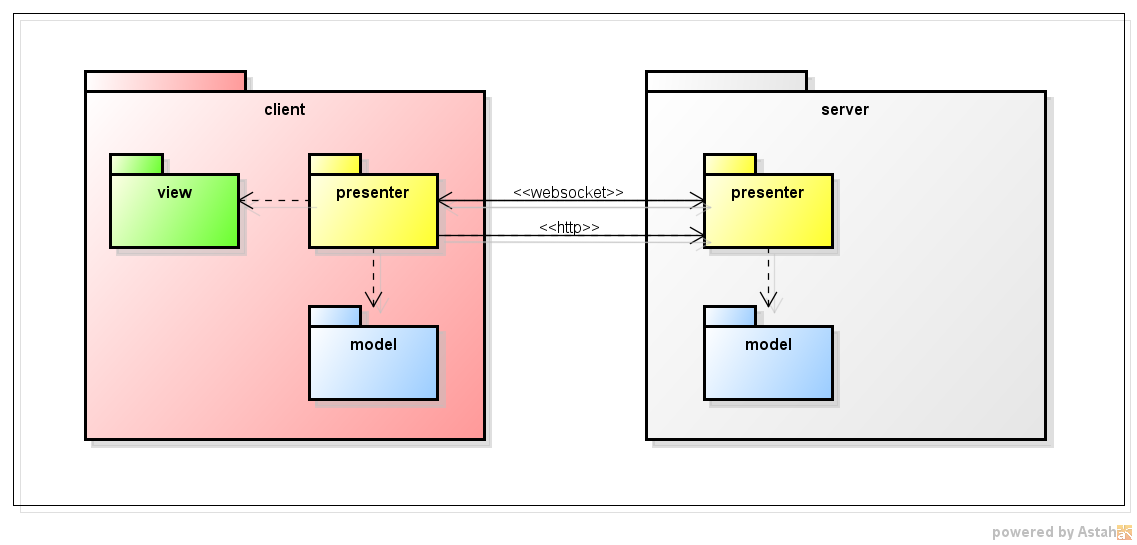
\includegraphics[width=%
\textwidth]
{./other/MVPIntroduzione.png} \caption{Diagramma UML architettura generale}
\end{figure}
\subsection{Diagrammi dei package}
Il seguente diagramma descrive le dipendenze intercorse fra i vari package\ped{G} del sistema Sequenziatore.
I diagrammi dei package |g| descrivono le dipendenze che intercorrono tra i vari
package\ped{G} che compongono il sistema.
Figura 3: Diagramma dei package del prodotto MyTalk.
Il sistema Sequenziatore è composto da due macro package\ped{G}:
\begin{enumerate}
	\item sequenziatore::client: le componenti di questo package\ped{G} realizzano la parte front-end\ped{G} del sistema Sequenziatore 
	\item sequenziatore::server: le componenti di questo package\ped{G} realizzano la parte back-end\ped{G} del sistema Sequenziatore 
\end{enumerate}
Il package\ped{G} sequenziatore.client è composto dai seguenti package\ped{G}:
\begin{itemize}
	\item sequenziatore::client::view;
	\item sequenziatore::client::presenter;
	\item sequenziatore::client::model.
\end{itemize}
Come è facilmente intuibile, la struttura del package\ped{G} sequenziatore.client si basa sulla struttura del design patter
architetturale Model View Presenter, scelto dal team Sirius per poter separare la logica di presentazione dei dati dalla logica di business.\\
I package\ped{G} che compongono il package\ped{G} sequenziatore::server sono:
\begin{itemize}
	\item sequenziatore::server::presenter;
	\item sequenziatore::server::model.
\end{itemize}
\subsubsection{Package sequenziatore::client::view}
Il package\ped{G} sequenziatore::client::view è composto da i seguenti package\ped{G}:
\begin{itemize}
	\item sequenziatore::client::view::process_owner: contiene le componenti template necessarie per la realizzazione dell’interfaccia grafica del process owner.
	\item sequenziatore::client::view::user: contiene le componenti template necessarie per la realizzazione dell’interfaccia grafica dell'user.
\end{itemize}
\subsubsection{Package sequenziatore::client::presenter}
Il package\ped{G} sequenziatore::client::presenter contiene tutte le componenti del Presenter della parte client\ped{G} del sistema Sequenziatore; ed è composto da i seguenti package\ped{G}:
\begin{itemize}
	\item sequenziatore::client::presenter::process_owner: contiene le componenti che costituiscono la componente Presenter
per il process owner, il package\ped{G} sequenziatore::client::presenter::process_owner è diviso ulteriormente nei sotto-package\ped{G}:
	\begin{itemize}
		\item sequenziatore::client::presenter::process_owner::views: contiene le classi necessarie per realizzare e gestire l'aggiornamento della parte grafica, usando i template presenti nel package\ped{g} sequenziatore::client::view::process_owner, e alla gestione degli eventi generati dall'interazione da parte del process owner con l'interfaccia grafica, gestendo inoltre la logica di business dell'applicazione;
	\end{itemize}
	\item sequenziatore::client::presenter::user: contiene le componenti che realizzano la componente Presenter per l'utente autenticato; i sotto-package\ped{G} di sequenziatore::client::presenter::user sono i seguenti:
	\begin{itemize}
		\item sequenziatore::client::presenter::user::views: contiene le classi necessarie per realizzare, mediante i template presenti nel package\ped{g} sequenziatore::client::view::user, l'interfaccia utente e gestirne l'interazione con l'utente autenticato, gestendo inoltre la logica di business dell'applicazione;
	\end{itemize}
\end{itemize}
\subsubsection{Package sequenziatore::client::model}
Il package\ped{G} sequenziatore::client::model contiene tutte le classi della componente Model. 
Il package\ped{G} sequenziatore::client::model contiene inoltre:
\begin{itemize}
	\item sequenziatore::client::model::collections contiene le varie collezioni di dati contenuti nel package model; il nome del package ricalca inoltre il nome del supertipo di tutte le collezioni di strutture date usate in un sistema sviluppato usando il framework\ped{G} Backbone.js\ped{G}
\end{itemize}

\section{Descrizione singoli componenti}%aka descrizione singole componenti
%inserire i vari view presenter model , ecc
\subsection{Package sequenziatore::server::presenter}
\paragraph{PresenterFacade}
	\begin{itemize}
		\item \textbf{Nome:} \texttt{PresenterFacade}
		\item \textbf{Tipo:} Abstract;
		\item \textbf{Package:} sequenziatore::server::presenter
		\item \textbf{Descrizione:} Classe astratta che ha il ruolo di decidere a che pacchetto inoltrare le richieste;
		\item \textbf{Relazione con altre componenti:} la classe richiama metodi delle classi:
		\begin{itemize}
			\item sequenziatore::server::presenter::iprocessowner::ProcessOwnerFacade;
			\item sequenziatore::server::presenter::iprocessowner::UserFacade.
		\end{itemize}
	\end{itemize}
%00000000000000000000000000000000000000000000000000000000000000000000000000000000000000000000000000000%
\subsubsection{Package sequenziatore::server::presenter::icommunication}
\paragraph{ICommunication}
	\begin{itemize}
		\item \textbf{Nome:} \texttt{ICommunication};
		\item \textbf{Tipo:} Interface;
		\item \textbf{Package:} sequenziatore::server::presenter::icommunication
		\item \textbf{Descrizione:} interfaccia che gestisce le comunicazioni con il \textit{presenter} lato \textit{client};
	\end{itemize}
%----------------------------------------------------------------------------------------------%
\paragraph{IDataFormatter}
	\begin{itemize}
		\item \textbf{Nome:} IDataFormatter;
		\item \textbf{Tipo:} Interface;
		\item \textbf{Package:} sequenziatore::server::presenter::icommunication
		\item \textbf{Descrizione:} interfaccia che gestisce le comunicazioni con il presenter lato \textit{client} tramite richieste http;
	\end{itemize}
%0000000000000000000000000000000000000000000000000000000000000000000000000000000000000000000000000%
\subsubsection{Package sequenziatore::server::presenter::communication}
\paragraph{HttpCommunication}
	\begin{itemize}
		\item \textbf{Nome:} \texttt{HttpCommunication};
		\item \textbf{Tipo:} Class;
		\item \textbf{Package:} sequenziatore::server::presenter::communication
		\item \textbf{Descrizione:} classe responsabile della gestione delle comunicazioni con il presenter lato \textit{client} tramite richieste http;
		\item \textbf{Relazione con altre componenti:} la classe implementa l' interfaccia :\texttt{sequenziatore::server::presenter::communication::ICommunication} e richiama metodi delle classi:
		\begin{itemize}
			\item sequenziatore::server::presenter::PresenterFacade.
		\end{itemize}
	\end{itemize}
%----------------------------------------------------------------------------------------------%
\paragraph{WebsocketCommunication}
	\begin{itemize}
		\item \textbf{Nome:} WebsocketCommunication;
		\item \textbf{Tipo:} Class;
		\item \textbf{Package:} sequenziatore::server::presenter::communication
		\item \textbf{Descrizione:} classe responsabile della gestione delle comunicazioni con il presenter lato \textit{client} tramite WebSocket;
		\item \textbf{Relazione con altre componenti:} la classe implementa l' interfaccia :\texttt{sequenziatore::server::presenter::communication::ICommunication} e richiama metodi delle classi:
		\begin{itemize}
			\item sequenziatore::server::presenter::PresenterFacade.
		\end{itemize}
	\end{itemize}
%----------------------------------------------------------------------------------------------%%deve stare prima di:1 e 2
\subsubsection{Package com.sirius.sequenziatore.server.presenter.user}
\paragraph{AccountController}
	\begin{itemize}
		\item \textbf{Nome:} \texttt{AccountController};
		\item \textbf{Package:} com.sirius.sequenziatore.server.presenter.user
		\item \textbf{Descrizione:} classe che permette la modifica dei dati di un utente come password o altre informazioni inerenti ai dettagli personali di un utente;
		\item \textbf{Relazione con altre componenti:} la classe richiama i metodi della classe:
		\begin{itemize}
			\item com.sirius.sequenziatore.server.model.IDataAccessObject;
		\end{itemize}
	\end{itemize}
%-----------------------------------------------------------------------------------------------%
\paragraph{UserProcessController}
	\begin{itemize}
		\item \textbf{Nome:} \texttt{UserProcessController};
		\item \textbf{Package:} com.sirius.sequenziatore.server.presenter.user
		\item \textbf{Descrizione:} classe che restituisce all' utente i dati di uno o più processi, può inoltre permettere l' inoltro della richiesta di un utente a iscriversi o disiscriversi a un processo;
		\item \textbf{Relazione con altre componenti:} la classe richiama i metodi della classe:
		\begin{itemize}
			\item com.sirius.sequenziatore.server.model.IDataAccessObject;
		\end{itemize}
	\end{itemize}
%-----------------------------------------------------------------------------------------------%
\paragraph{UserStepController}
	\begin{itemize}
		\item \textbf{Nome:} \texttt{UserStepController};
		\item \textbf{Package:} com.sirius.sequenziatore.server.presenter.user
		\item \textbf{Descrizione:} Gestisce l' esecuzione di un passo da parte di un utente inoltrando la richiesta di inserire i dati nel \textit{database} e in caso sia richiesto, notifica l' amministratore che deve controllare se il passo è stato completato, inoltre è incaricato di restituire i dati inseriti di un passo quando richiesto da un utente;
		\item \textbf{Relazione con altre componenti:} la classe richiama i metodi della classe:
		\begin{itemize}
			\item com.sirius.sequenziatore.server.model.IDataAccessObject;
		\end{itemize}
	\end{itemize}
%-----------------------------------------------------------------------------------------------%
\paragraph{ReportController}
	\begin{itemize}
		\item \textbf{Nome:} \texttt{ReportController};
		\item \textbf{Package:} com.sirius.sequenziatore.server.presenter.user
		\item \textbf{Descrizione:} Classe che fornisce i dati per generare il report dell' utente riferito al processo richiesto;
		\item \textbf{Relazione con altre componenti:} la classe implementa l' interfaccia sequenziatore.server.presenter.iuser.IReport e richiama i metodi della classe:
		\begin{itemize}
			\item com.sirius.sequenziatore.server.model.IDataAccessObject;
		\end{itemize}
	\end{itemize}
%-----------------------------------------------------------------------------------------------%             %1
\subsubsection{Package sequenziatore::server::presenter::iprocessowner}
\paragraph{IProcessManager}
	\begin{itemize}
		\item \textbf{Nome:} \texttt{IProcessManager};
		\item \textbf{Package:} sequenziatore::server::presenter::iprocessowner
		\item \textbf{Descrizione:} Interfaccia che permette la gestione dei processi al \textit{process owner};
	\end{itemize}

%----------------------------------------------------------------------------------------------%

\paragraph{IStepManager}
	\begin{itemize}
		\item \textbf{Nome:} \texttt{IStepManager};
		\item \textbf{Package:} sequenziatore::server::presenter::iprocessowner
		\item \textbf{Descrizione:} Interfaccia che permette la gestione dei passi al \textit{process owner};
	\end{itemize}

%----------------------------------------------------------------------------------------------%
\paragraph{IUserManager}
	\begin{itemize}
		\item \textbf{Nome:} \texttt{IUserManager};
		\item \textbf{Package:} sequenziatore::server::presenter::iprocessowner
		\item \textbf{Descrizione:} Interfaccia per la gestione degli utenti iscritti ai processi;
	\end{itemize}
%----------------------------------------------------------------------------------------------%

\paragraph{IReport}
	\begin{itemize}
		\item \textbf{Nome:} \texttt{IReport};
		\item \textbf{Package:} sequenziatore::server::presenter::iprocessowner
		\item \textbf{Descrizione:} Interfaccia che permette la gestione dei report al \textit{process owner};
	\end{itemize}

%0000000000000000000000000000000000000000000000000000000000000000000000000000000000000000000000000%
\subsubsection{Package sequenziatore::server::presenter::processowner}

\paragraph{ProcessManager}
	\begin{itemize}
		\item \textbf{Nome:} \texttt{ProcessManager};
		\item \textbf{Package:} sequenziatore::server::presenter::processowner
		\item \textbf{Descrizione:} Classe che riceve le richieste del \textit{process owner} per la gestione dei processi come creazione,modifica e eliminazione degli stessi;
		\item \textbf{Relazione con altre componenti:} la classe implementa l' intefaccia sequenziatore::server::presenter::iprocessowner::IProcessManager ed invoca i metodi delle classi:
		\begin{itemize}
			\item \textcolor{red}{manca}
		\end{itemize}
	\end{itemize}
%----------------------------------------------------------------------------------------------%
\paragraph{StepManager}
	\begin{itemize}
		\item \textbf{Nome:} \texttt{StepManager};
		\item \textbf{Package:} sequenziatore::server::presenter::processowner
		\item \textbf{Descrizione:} Classe che permette l' elaborazione delle richieste del \textit{process owner} per quanto concerne la creazione,la rimozione e la modifica di passi;
		\item \textbf{Relazione con altre componenti:} la classe implementa l' intefaccia sequenziatore::server::presenter::iprocessowner::IStepManager ed invoca i metodi delle classi:
		\begin{itemize}
			\item \textcolor{red}{manca}
		\end{itemize}
	\end{itemize}
	%----------------------------------------------------------------------------------------------%
\paragraph{UserManager}
	\begin{itemize}
		\item \textbf{Nome:} \texttt{UserManager};
		\item \textbf{Package:} sequenziatore::server::presenter::iprocessowner
		\item \textbf{Descrizione:} Classe che permette la gestione degli utenti iscritti alla piattaforma, permettendogli di rimuovere utenti da processi,;
		\item \textbf{Relazione con altre componenti:} la classe implementa l' intefaccia sequenziatore::server::presenter::iprocessowner::IUserManager ed invoca i metodi delle classi:
		\begin{itemize}
			\item \textcolor{red}{manca}
		\end{itemize}
	\end{itemize}

%----------------------------------------------------------------------------------------------%
\paragraph{Report}
	\begin{itemize}
		\item \textbf{Nome:} \texttt{Report};
		\item \textbf{Package:} sequenziatore::server::presenter::iprocessowner
		\item \textbf{Descrizione:} Classe che permette la gestione delle richieste dei report al \textit{process owner}, permettendogli di visualizzare i risultati raggiunti in un processo;
		\item \textbf{Relazione con altre componenti:} la classe implementa l' intefaccia sequenziatore::server::presenter::iprocessowner::IReport ed invoca i metodi delle classi:
		\begin{itemize}
			\item \textcolor{red}{manca}
		\end{itemize}
	\end{itemize}
   %2
\subsection{Package sequenziatore::server::model}
\paragraph{DaoFacade}
	\begin{itemize}
		\item \textbf{Nome:} \texttt{DaoFacade};
		\item \textbf{Tipo:} abstract;
		\item \textbf{Package:} sequenziatore::server::model
		\item \textbf{Descrizione:} Classe astratta che decide a che pacchetto assegnare la richiesta di esecuzione \textit{query};
		\item \textbf{Relazione con altre componenti:} la classe invoca i metodi delle seguenti classi:
		\begin{itemize}
			\item sequenziatore::server::model::daoprocessowner::ObjectTransfer tramite l' interfaccia sequenziatore::server::model::daoprocessowner::IObjectTransfer
			\item sequenziatore::server::model::daoprocessowner::DataAccessObject tramite l' interfaccia sequenziatore::server::model::daoprocessowner::IDataAccessObject
			\item sequenziatore::server::model::daostep::ObjectTransfer tramite l' interfaccia sequenziatore::server::model::daostep::IObjectTransfer
			\item sequenziatore::server::model::daostep::DataAccessObject tramite l' interfaccia sequenziatore::server::model::daostep::IDataAccessObject
			\item sequenziatore::server::model::daouser::ObjectTransfer tramite l' interfaccia sequenziatore::server::model::daouser::IObjectTransfer
			\item sequenziatore::server::model::daouser::DataAccessObject tramite l' interfaccia sequenziatore::server::model::daouser::IDataAccessObject
			\item sequenziatore::server::model::daoprocess::ObjectTransfer tramite l' interfaccia sequenziatore::server::model::daoprocess::IObjectTransfer
			\item sequenziatore::server::model::daoprocess::DataAccessObject tramite l' interfaccia sequenziatore::server::model::daoprocess::IDataAccessObject
		\end{itemize}
	\end{itemize}
\subsubsection{Package sequenziatore::server::model::daouser}
\paragraph{IDataAccessObject}
	\begin{itemize}
		\item \textbf{Nome:} \texttt{IDataAccessObject};
		\item \textbf{Package:} sequenziatore::server::model::daouser
		\item \textbf{Descrizione:} Interfaccia con il compito di interagire con il database.
	\end{itemize}
%------------------------------------------------------------------------------%
\paragraph{DataAccessObject}
	\begin{itemize}
		\item \textbf{Nome:} \texttt{DataAccessObject};
		\item \textbf{Package:} sequenziatore::server::model::daouser
		\item \textbf{Descrizione:} classe che si occupa di effettuare le richieste al database, acquisendo i dati richiesti o inserendone di nuovi.
		\item \textbf{Relazione con altre componenti:} la classe implementa l' interfaccia sequenziatore::server::model::daouser::IDataAccessObject ed invoca metodi delle classi:
		\begin{itemize}
			\item sequenziatore::server::model::daouser::ObjectTransfer tramite l' interfaccia sequenziatore::server::model::daouser::IObjectTransfer
		\end{itemize}
	\end{itemize}
	%------------------------------------------------------------------------------%
\paragraph{IObjectTransfer}
	\begin{itemize}
		\item \textbf{Nome:} \texttt{IObjectTransfer};
		\item \textbf{Package:} sequenziatore::server::model::daouser
		\item \textbf{Descrizione:} Interfaccia che permette lo scambio di dati tra model e presenter.
	\end{itemize}
	%------------------------------------------------------------------------------%
\paragraph{ObjectTransfer}
	\begin{itemize}
		\item \textbf{Nome:} \texttt{ObjectTransfer};
		\item \textbf{Package:} sequenziatore::server::model::daouser
		\item \textbf{Descrizione:} Classe che permette lo scambio di dati tra la classe DataAccessObject e il presenter.
		\item \textbf{Relazione con altre componenti:} la classe implementa l'interfaccia sequenziatore::server::model::daouser::IObjectTransfer.
	\end{itemize}
%000000000000000000000000000000000000000000000000000000000000000000000000000000000000%
\subsubsection{Package sequenziatore::server::model::daoprocessowner}
\paragraph{IDataAccessObject}
	\begin{itemize}
		\item \textbf{Nome:} \texttt{IDataAccessObject};
		\item \textbf{Package:} sequenziatore::server::model::daoprocessowner
		\item \textbf{Descrizione:} Interfaccia con il compito di interagire con il database.
	\end{itemize}
	%------------------------------------------------------------------------------%
\paragraph{DataAccessObject}
\begin{itemize}
		\item \textbf{Nome:} \texttt{DataAccessObject};
		\item \textbf{Package:} sequenziatore::server::model::daoprocessowner
		\item \textbf{Descrizione:} classe che si occupa di effettuare le richieste al database, acquisendo i dati richiesti o inserendone di nuovi.
		\item \textbf{Relazione con altre componenti:} la classe implementa l' interfaccia sequenziatore::server::model::daoprocessowner::IDataAccessObject ed invoca metodi delle classi:
		\begin{itemize}
			\item sequenziatore::server::model::daoprocessowner::ObjectTransfer tramite l' interfaccia sequenziatore::server::model::daoprocessowner::IObjectTransfer
		\end{itemize}
\end{itemize}
	%------------------------------------------------------------------------------%
\paragraph{IObjectTransfer}
	\begin{itemize}
		\item \textbf{Nome:} \texttt{IObjectTransfer};
		\item \textbf{Package:} sequenziatore::server::model::daoprocessowner
		\item \textbf{Descrizione:} Interfaccia che permette lo scambio di dati tra model e presenter.
	\end{itemize}
	%------------------------------------------------------------------------------%
\paragraph{ObjectTransfer}
	\begin{itemize}
		\item \textbf{Nome:} \texttt{ObjectTransfer};
		\item \textbf{Package:} sequenziatore::server::model::daoprocessowner
		\item \textbf{Descrizione:} Classe che permette lo scambio di dati tra la classe DataAccessObject e il presenter.
		\item \textbf{Relazione con altre componenti:} la classe implementa l'interfaccia sequenziatore::server::model::daoprocessowner::IObjectTransfer.
	\end{itemize}
%000000000000000000000000000000000000000000000000000000000000000000000000000000000000%
\subsubsection{Package sequenziatore::server::model::daoprocess}
\paragraph{IDataAccessObject}
	\begin{itemize}
		\item \textbf{Nome:} \texttt{IDataAccessObject};
		\item \textbf{Package:}sequenziatore::server::model::daoprocess
		\item \textbf{Descrizione:} Interfaccia con il compito di interagire con il database.
	\end{itemize}
	%------------------------------------------------------------------------------%
\paragraph{DataAccessObject}
	\begin{itemize}
		\item \textbf{Nome:} \texttt{DataAccessObject};
		\item \textbf{Package:} sequenziatore::server::model::daoprocess
		\item \textbf{Descrizione:} classe che si occupa di effettuare le richieste al database, acquisendo i dati richiesti o inserendone di nuovi.
		\item \textbf{Relazione con altre componenti:} la classe implementa l' interfaccia sequenziatore::server::model::daoprocess::IDataAccessObject ed invoca metodi delle classi:
		\begin{itemize}
			\item sequenziatore::server::model::daoprocess::ObjectTransfer tramite l' interfaccia sequenziatore::server::model::daoprocess::IObjectTransfer
	\end{itemize}
\end{itemize}
	%------------------------------------------------------------------------------%
\paragraph{IObjectTransfer}
	\begin{itemize}
		\item \textbf{Nome:} \texttt{IObjectTransfer};
		\item \textbf{Package:} sequenziatore::server::model::daoprocess
		\item \textbf{Descrizione:} Interfaccia che permette lo scambio di dati tra model e presenter.
	\end{itemize}
	%------------------------------------------------------------------------------%
\paragraph{ObjectTransfer}
	\begin{itemize}
		\item \textbf{Nome:} \texttt{ObjectTransfer};
		\item \textbf{Package:} sequenziatore::server::model::daoprocess
		\item \textbf{Descrizione:} Classe che permette lo scambio di dati tra la classe DataAccessObject e il presenter.
		\item \textbf{Relazione con altre componenti:} la classe implementa l'interfaccia sequenziatore::server::model::daoprocess::IObjectTransfer.
	\end{itemize}
%000000000000000000000000000000000000000000000000000000000000000000000000000000000000%
\subsubsection{Package sequenziatore::server::model::daostep}
\paragraph{IDataAccessObject}
	\begin{itemize}
		\item \textbf{Nome:} \texttt{IDataAccessObject};
		\item \textbf{Package:} sequenziatore::server::model::daostep
		\item \textbf{Descrizione:} Interfaccia con il compito di interagire con il database.
	\end{itemize}
	%------------------------------------------------------------------------------%
\paragraph{DataAccessObject}
	\begin{itemize}
		\item \textbf{Nome:} \texttt{DataAccessObject};
		\item \textbf{Package:} sequenziatore::server::model::daostep
		\item \textbf{Descrizione:} classe che si occupa di effettuare le richieste al database, acquisendo i dati richiesti o inserendone di nuovi.
		\item \textbf{Relazione con altre componenti:} la classe implementa l' interfaccia sequenziatore::server::model::daostep::IDataAccessObject ed invoca metodi delle classi:
		\begin{itemize}
			\item sequenziatore::server::model::daostep::ObjectTransfer tramite l' interfaccia sequenziatore::server::model::daostep::IObjectTransfer
	\end{itemize}
	\end{itemize}
	%------------------------------------------------------------------------------%
\paragraph{IObjectTransfer}
	\begin{itemize}
		\item \textbf{Nome:} \texttt{IObjectTransfer};
		\item \textbf{Package:} sequenziatore::server::model::daostep
		\item \textbf{Descrizione:} Interfaccia che permette lo scambio di dati tra model e presenter.
	\end{itemize}
	%------------------------------------------------------------------------------%
\paragraph{ObjectTransfer}
	\begin{itemize}
		\item \textbf{Nome:} \texttt{ObjectTransfer};
		\item \textbf{Package:} sequenziatore::server::model::daostep
		\item \textbf{Descrizione:} Classe che permette lo scambio di dati tra la classe DataAccessObject e il presenter.
		\item \textbf{Relazione con altre componenti:} la classe implementa l'interfaccia sequenziatore::server::model::daostep::IObjectTransfer.
	\end{itemize}
\section{Design pattern}

\subsection{Design pattern architetturali}

\subsubsection{Model View Presenter}
\begin{itemize}
\item \textbf{Scopo:}
Il \textit{pattern\ped{G}} architetturale \textit{Model View Presenter} (MVP) è un derivato del \textit{Model View Controller} (MVC), focalizzato sulla valorizzazione della logica della presentazione. Entrambi i pattern hanno lo sopo di disaccoppiare la logica dell'applicazione dalla rappresentazione grafica.\\
Il \textit{pattern\ped{G}} MVP prevede la suddivisione dell'applicazione in tre componenti:
\begin{itemize}
\item \textbf{Model:} Definisce il modello dati e le regole di accesso e di modifica;
\item \textbf{View:} Si occupa della rappresentazione dell'interfaccia utente;
\item \textbf{Presenter:} Contiene la logica dell'applicazione, si occupa delle comunicazioni tra vista e modello e dell'aggiornamento della vista.
\end{itemize}

\item \textbf{Contesto d'uso:}
\end{itemize}

\subsection{Design pattern strutturali}
\subsubsection{Adapter}
\begin{itemize}
\item \textbf{Scopo:}
Il \textit{pattern\ped{G}} strutturale \textit{Adapter} permette di utilizzare un componente software la cui interfaccia deve essere adattata per potersi integrare ad un'altra presente nell'applicazione esistente.\\
Tale \textit{pattern\ped{G}} può essere basato sia su classi che su oggetti, perciò, l'istanza della classe da adattare, può derivare tramite ereditarietà o composizione.

\item \textbf{Contesto d'uso:}
\end{itemize}

\subsubsection{Decorator}
\begin{itemize}
\item \textbf{Scopo:}
Il \textit{pattern\ped{G}} strutturale \textit{Decorator} permette di aggiungere dinamicamente funzionalità ad un oggetto base, con la possibilità di comporle arbitrariamente.\\
Tale \textit{pattern\ped{G}} si pone come alternativa all'uso dell'ereditarietà singola o multipla;

\item \textbf{Contesto d'uso:}
\end{itemize}

\subsubsection{Facade}
\begin{itemize}
\item \textbf{Scopo:}
Il \textit{pattern\ped{G}} strutturale \textit{Facade} prevede l'utilizzo di un'interfaccia unica e semplice per un sottosistema complesso, diminuendo la complessità del sistema;

\item \textbf{Contesto d'uso:}
\end{itemize}

\subsubsection{Proxy}
\begin{itemize}
\item \textbf{Scopo:}
Il \textit{pattern\ped{G}} strutturale \textit{Proxy} viene utilizzato per accedere ad un un oggetto complesso di cui si vogliono controllare gli accessi, tramite un oggetto semplice, che espone gli stessi metodi dell'oggetto che maschera;

\item \textbf{Contesto d'uso:}
\end{itemize}

\subsection{Design pattern creazionali}
\subsubsection{Singleton}
\begin{itemize}
\item \textbf{Scopo:}
Il \textit{pattern\ped{G}} creazionale \textit{Singleton} viene utilizzato quando si ha la necessità di avere una sola istanza di una classe e di avere un punto di accesso globale ad essa;

\item \textbf{Contesto d'uso:}
\end{itemize}

\subsubsection{Abstract Factory}
\begin{itemize}
\item \textbf{Scopo:}
Il \textit{pattern\ped{G}} creazionale \textit{Abstract Factory} fornisce un'interfaccia per creare famiglie di prodotti senza specificare classi concrete. Le classi che concretizzano tale interfaccia, vengono costruite una sola volta, e consentono di utilizzare una varietà di elementi che presentano le stesse funzionalità con diverse implementazioni;

\item \textbf{Contesto d'uso:}
\end{itemize}

\subsection{Design pattern comportamentali}
\subsubsection{Command}
\begin{itemize}
\item \textbf{Scopo:}
Il \textit{pattern\ped{G}} comportamentale \textit{Command} permette di separare l'invocazione di un comando dai suoi dettagli implementativi;

\item \textbf{Contesto d'uso:}
\end{itemize}

\subsubsection{Iterator}
\begin{itemize}
\item \textbf{Scopo:}
Il \textit{pattern\ped{G}} comportamentale \textit{Iterator} fornisce l'accesso sequenziale agli elementi di un aggregato senza esporne l'implementazione;

\item \textbf{Contesto d'uso:}
\end{itemize}

\subsubsection{Observer}
\begin{itemize}
\item \textbf{Scopo:}
Il \textit{pattern\ped{G}} comportamentale \textit{Observer} viene utilizzato quando si vuole realizzare una dipendenza tra un soggetto e più oggetti, in cui il cambiamento di stato del un soggetto, viene notificato a tutti gli oggetti dipendenti;

\item \textbf{Contesto d'uso:}
\end{itemize}

\subsubsection{Strategy}
\begin{itemize}
\item \textbf{Scopo:}
Il \textit{pattern\ped{G}} comportamentale \textit{Strategy} viene utilizzato per definire una famiglia di algoritmi, incapsularli e renderli intercambiabili;

\item \textbf{Contesto d'uso:}
\end{itemize}

\subsubsection{Template method}
\begin{itemize}
\item \textbf{Scopo:}
Il \textit{pattern\ped{G}} comportamentale \textit{Template method} viene utilizzato per definire lo scheletro di un algoritmo, lasciando l'implementazione di alcuni passi alle sottoclassi. In particolare consente di specificare l'ordine delle operazioni da effettuare ma di delegare la loro implementazione o parte di essa alle sottoclassi;

\item \textbf{Contesto d'uso:}
\end{itemize}
\end{document}